\section{Estado del Arte}

\subsection{2.1 Antenas para constelaciones LEO}

Aunque los reflectores parabólicos dominaron durante décadas las estaciones terrestres satelitales, su rigidez mecánica los vuelve poco prácticos ante la densidad y velocidad de las constelaciones LEO actuales. Particularmente llamativo es el hecho de que los phased-array multibean han ganado terreno de forma acelerada precisamente por su capacidad de generar y rastrear múltiples haces de forma electrónica. 

He et al. ofrecen una revisión exhaustiva que subraya cómo estos arrays permiten soportar simultáneamente varios satélites en vista, algo esencial para el handover fluido y la gestión de tráfico masivo \cite{He2021}. En muchos casos estudiados, sin embargo, las limitaciones en cobertura hemisférica y los altos costos de los elementos radiantes tienden a restringir su despliegue masivo. No obstante, cabe matizar que las arquitecturas conformes y distribuidas están mitigando progresivamente estas barreras, especialmente en terminales tanto terrestres como embarcadas.

Resulta revelador observar que el salto desde soluciones mecánicas a electrónicas no solo reduce latencia de rastreo, sino que habilita funcionalidades antes impensables, como beamforming adaptativo en entornos con múltiples usuarios.

\subsection{2.2 Diseños en bandas L y S}

Uno de los desafíos persistentes al trabajar en bandas L y S radica en equilibrar ganancia, ancho de banda y tamaño de apertura. Lejos de ser un asunto resuelto, los diseños de apertura compartida dual-frecuencia representan un avance notable para plataformas con restricciones volumétricas como CubeSats. 

Zhao et al. proponen una solución shared-aperture de haz ancho específicamente orientada a comunicaciones LEO, donde el compromiso entre beamwidth y eficiencia radiativa se maneja mediante topologías híbridas que mantienen buen desempeño en ambas bandas \cite{Zhao2024}. Diseños helicoidales desplegables, por su parte, destacan en escenarios que requieren alta ganancia con bajo peso, aunque suelen sacrificar flexibilidad en escaneo electrónico. 

En la práctica, las arquitecturas patch multibanda y arrays conformes tienden a ofrecer mejor adaptabilidad para enlaces asimétricos típicos de sensores IoT, si bien introducen complejidades en acoplamiento y eficiencia de potencia.


\begin{table*}[htbp]
\renewcommand{\arraystretch}{1.3} % Mantiene el espaciado vertical estándar de IEEE
\centering
\caption{\textsc{Comparación de Características Principales entre Bandas L y S para Enlaces LEO-IoT Ambientales}}
\label{tab:comparacion_bandas_leo}
% \columnwidth obliga a la tabla a ocupar exactamente el ancho del margen de la columna
\begin{tabularx}{\columnwidth}{|X|c|c|}
\hline
\textbf{Parámetro} & \textbf{Banda L} & \textbf{Banda S} \\ \hline
Frecuencia típica & 1-2 GHz & 2-4 GHz \\ \hline
Penetración atmosférica & Excelente & Buena \\ \hline
Ancho de banda disponible & Moderado & Mayor \\ \hline
Tamaño de antena requerido & Mayor & Menor \\ \hline
Sensibilidad a Doppler & Menor & Moderada \\ \hline
\end{tabularx}
\end{table*}

\subsection{2.3 Aplicaciones en monitoreo ambiental}

Resulta especialmente interesante cómo las promesas de conectividad global directa chocan con las realidades operativas del monitoreo ambiental distribuido. Akar et al., en su tutorial sobre DtS-IoT, exponen con claridad las arquitecturas donde dispositivos de muy bajo consumo transmiten directamente a satélites LEO, eliminando gateways terrestres intermedios \cite{Akar2026}. 

Esta aproximación resulta particularmente atractiva para zonas remotas —bosques tropicales, regiones polares o áreas oceánicas— donde el despliegue de infraestructura tradicional resulta inviable. Aun así, persisten brechas importantes: la mayoría de los estudios se centran en viabilidad de enlace genérica, dejando relativamente poco espacio al análisis específico de requisitos de antena para flujos esporádicos y de baja tasa propios de sensores ambientales.

\begin{figure}[h]
\centering
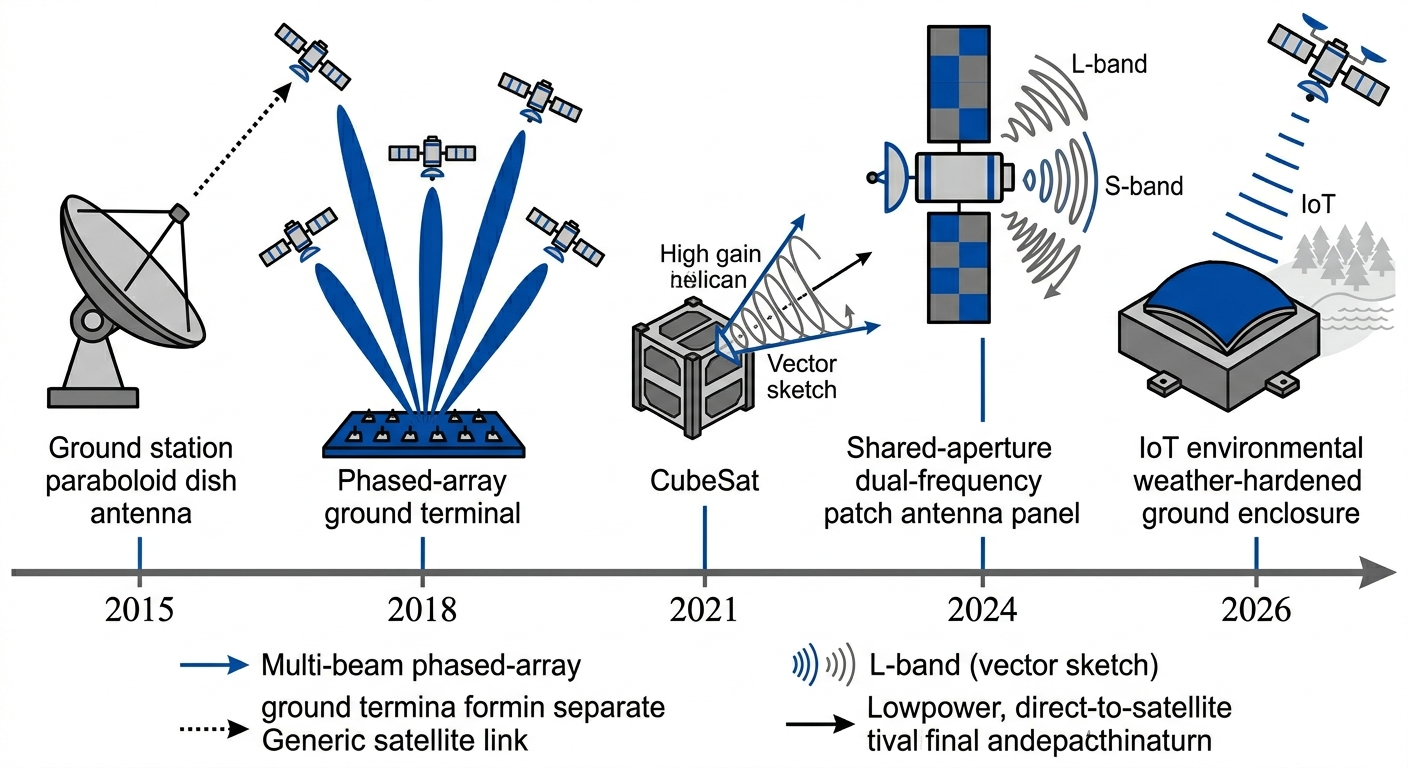
\includegraphics[width=\linewidth]{fig2.png}
\caption{Evolución temporal de arquitecturas de antena para constelaciones LEO (2015-2026), destacando transición desde reflectores a phased-array, shared-aperture y soluciones conformes específicas para IoT ambiental.}
\label{fig:temporal_evolution}
\end{figure}

Las brechas identificadas apuntan hacia la necesidad de diseños híbridos que optimicen simultáneamente eficiencia energética, robustez ante Doppler y cobertura en entornos de propagación desafiantes. Este trabajo busca contribuir precisamente en esa intersección entre estado del arte tecnológico y demandas prácticas del monitoreo ambiental.